%==============================================================================
% ModelCrew · CUMCM 国赛论文模板（中文，ctex，自包含）
%   编译：  latexmk -xelatex 6_paper.tex   （含中文，建议 XeLaTeX）
%   占位符已全部替换；数字与 6_paper.md / frozen_numbers.json 同源。
%   已用 MiKTeX xelatex 编译通过 → 6_paper.pdf（13 页，无未定义引用）。复现：xelatex 6_paper.tex（跑两遍）。
%==============================================================================
\documentclass[12pt,a4paper]{ctexart}

\usepackage[margin=2.5cm]{geometry}
\usepackage{amsmath,amssymb}
\usepackage{graphicx}
\usepackage{booktabs}
\usepackage{titlesec}
\usepackage{abstract}
\usepackage[hidelinks]{hyperref}

\title{\textbf{应急调度策略 A/B 的公平比较：Simpson 反转的识别与混杂校正}}
\author{}
\date{}

\begin{document}

%------------------------------------------------------------------ 承诺页（占位）
\thispagestyle{empty}
\noindent （演示案例，承诺书略）
\newpage

%------------------------------------------------------------------ 摘要页
\maketitle
\vspace{-2em}
\begin{center}\textbf{\large 摘\quad 要}\end{center}
\noindent
针对某市两套应急调度派遣策略 A、B 的优劣评估问题，本文基于 700 条出警记录（字段：策略 \texttt{policy}、呼叫严重度 \texttt{severity}、是否按时到达 \texttt{on\_time}），建立``描述 $\to$ 质疑 $\to$ 校正''三层递进的统计分析框架，识破合并率陷阱并给出可落地的公平比较方案。

\textbf{针对问题一（哪套按时率更高）}，本文建立\textbf{边际（合并）率比较模型}，用两比例差 $z$ 检验求解，得合并按时率 A 为 0.8286、B 为 0.5200，率差 $+30.86$ 个百分点（95\% CI $[24.30,37.41]$ pp，$p<10^{-15}$）。表面看 A 远高于 B；但本文随即论证：\textbf{此结论是混杂误导的陷阱，不可据此向市政推荐 A}——这正是题目设计的反面教材。

\textbf{针对问题二（结论是否可靠、有无混杂误判）}，本文建立\textbf{分层比较模型}并提出可证伪的 \textbf{Simpson 反转判定准则}（合并方向与每个层内方向均相反即成立），按 \texttt{severity} 分层求解。结果：合并口径 A 高，但\textbf{轻案层 B 0.94 $>$ A 0.90、重案层 B 0.45 $>$ A 0.40，两层方向一致地 B 高}，反转判定为真。混杂机制清楚：A 仅 14.3\% 接重案、B 高达 85.7\% 接重案（失衡 6.0 倍），合并率把``案件难度差''误算成``策略效果差''。这是教科书级 Simpson 悖论在本数据上的真实发生。

\textbf{针对问题三（公平比较的正确做法与落地建议）}，本文以\textbf{直接标准化率差}为主、\textbf{Mantel--Haenszel 合并 OR} 与 \textbf{logistic 回归}为印证，三法交叉校正 \texttt{severity}。求解得：标准化率差（总体权）B 较 A 优 $+4.5$ pp（95\% bootstrap CI $[-3.83,+12.67]$ pp）、MH-OR(A/B)$=0.7527$（95\% CI $[0.4378,1.2941]$）、logistic 校正 OR(B/A)$=1.323$（95\% CI $[0.7728,2.265]$，$p=0.31$）。\textbf{三法点估计方向一致地指向 B 略优}。但须如实指出：\textbf{三法的 95\% 区间均跨过各自零值（率差含 0、OR 含 1、$p>0.05$），效应未达统计显著}。故本案最强且唯一可防守的结论是：\textbf{在给定可观测严重度下，校正后 B 不劣于 A、点估计略优约 4--5 pp，但在 $n=700$、最小格 $n=50$ 下尚不足以判定``B 显著更优''；而``用合并率推荐 A''几乎确定是错误方向}。

\textbf{灵敏度方面}，标准化率差在总体权 / A 人群权 / B 人群权三套权重下恒为负（B 优），漂移仅约 0.7 pp，方向对权重稳健；Breslow--Day（$p=0.615$）与 logistic 交互项（$p=0.617$）均不显著，层间效应同质，支持合并 OR；bootstrap 重跑数值逐位可复现。

\textbf{本文创新点}在于把``公平''操作化为``同等案件难度下比较''，提出可向市政一句话讲清的``\textbf{难度配平比较法}（severity-matched fair comparison）''，并以流行病学的人口标准化作类比；同时全程严守``方向 $\neq$ 显著、相关 $\neq$ 因果''的措辞红线，不把点估计优势夸大为显著优势或因果效应。

\vspace{1em}
\noindent\textbf{关键词：} Simpson 悖论；混杂校正；直接标准化率；Mantel--Haenszel 合并 OR；logistic 回归

\newpage
\tableofcontents
\newpage

%------------------------------------------------------------------ 正文
\section{问题重述}
某市试点两套应急调度派遣策略 A 与 B，在一段时期内记录了每次出警的三个字段：本次采用的策略 \texttt{policy}（A / B）、呼叫严重度 \texttt{severity}（Low 轻 / High 重）、是否在目标时限内到达 \texttt{on\_time}（1 是 / 0 否）。数据为 \texttt{data/dispatch.csv}，共 700 行，由确定性脚本生成、字节级可复现。要求回答：

\begin{itemize}
\item \textbf{Q1}：哪套策略的``按时到达率''更高？应向市政推荐哪一套？
\item \textbf{Q2}：这个结论可靠吗？是否存在混杂导致的误判？
\item \textbf{Q3}：若要公平比较两套策略，正确的做法是什么？给出可落地建议。
\end{itemize}

用自己的话归纳，本题的实质并非``算一个率''，而是\textbf{识破合并率在混杂下的误导，给出剔除混杂后可信的策略比较与落地建议}。三问层层递进（描述 Q1 $\to$ 质疑 Q2 $\to$ 校正 Q3）构成一条自纠链：Q1 的``直觉答案''预期与 Q3 的``正确方向''相反，这是题目考点而非数据错误。变量角色：\texttt{policy} 是处理变量（treatment），\texttt{on\_time} 是结果变量（outcome），\texttt{severity} 是疑似混杂（confounder）——它既可能影响``用哪套策略''，又直接影响``是否按时''。

\section{问题分析与基本假设}
\subsection{问题分析}
核心判断是 \texttt{severity} 同时关联处理与结果，构成混杂结构：若不控制它，合并率会把``案件难度差''误当``策略效果差''。因此分析路径定为三层：先给 Q1 的合并率作为``陷阱基线''；用分层检验混杂是否真导致反转（Q2）；用标准化 / 合并 OR / 回归三法在控制 \texttt{severity} 后做公平比较（Q3）。是否真混杂、反转是否真发生，均由数据实证，不预设。

\subsection{基本假设（每条含理由与代价）}
\begin{itemize}
\item \textbf{A1}：\texttt{severity} 是唯一相关、可控的混杂。理由：数据仅 3 字段。代价：现实可能有时段/路况/警力等\textbf{未观测混杂}，本数据无法测——结论只能限定在``给定可观测变量''下，\textbf{不可声称因果}。
\item \textbf{A2}：每行是一次独立出警，可直接计数算率。理由：\texttt{call\_id} 1..700 唯一连续、无重复。代价：若存在时间自相关，CI 偏窄。
\item \textbf{A3}：\texttt{on\_time} 口径在 A、B 间一致。理由：题面把 \texttt{on\_time} 当统一结果字段。代价：若两策略各自定义时限则不可比；数据内无法验证。
\item \textbf{A4}：样本对该市出警总体有代表性。理由：题面要求向市政推荐。代价：试点期记录可能有\textbf{选择偏差}，外推受限。
\item \textbf{A5}：\texttt{severity} 划分客观、两策略间含义一致。理由：作为分层依据必须可比。代价：若 \texttt{severity} 判定内生于 \texttt{policy}，分层/标准化失效；数据内无法验证。
\item \textbf{A6}：二值结果用率 / 卡方 / logistic 即可。理由：无时间戳、无机理过程。代价：若关心响应时间分布则丢信息。
\end{itemize}
A1、A5 是最该被质疑、也最关键的两条，下文模型评价中如实写入其不可验证性。

\section{符号说明}
\begin{center}
\begin{tabular}{ll}
\toprule
符号 & 含义 \\
\midrule
$T\in\{A,B\}$ & 处理变量（policy） \\
$S\in\{L,H\}$ & 混杂变量（severity：Low / High） \\
$Y\in\{0,1\}$ & 结果变量（on\_time） \\
$n_{ts}$ & 策略 $t$、层 $s$ 的样本数 \\
$y_{ts}$ & 策略 $t$、层 $s$ 的按时数 \\
$\hat p_{ts}=y_{ts}/n_{ts}$ & 层内按时率 \\
$\hat p_t$ & 策略 $t$ 的合并（边际）按时率 \\
$w_s$ & 标准化层权重（$w_L+w_H=1$） \\
$\hat p_t^{\text{std}}=\sum_s w_s\hat p_{ts}$ & 标准化率 \\
$\widehat{OR}_{MH}$ & Mantel--Haenszel 合并比值比 \\
$\beta_1$ & logistic 中 B 相对 A 的对数几率差（控制 $S$） \\
\bottomrule
\end{tabular}
\end{center}

锁定的单元计数（数据实测）：

\begin{center}
\begin{tabular}{lccccc}
\toprule
 & $n_{tL}$ & $\hat p_{tL}$ & $n_{tH}$ & $\hat p_{tH}$ & 合并率 $\hat p_t$ \\
\midrule
A & 300 & 0.9000 & 50 & 0.4000 & 0.8286 \\
B & 50 & 0.9400 & 300 & 0.4500 & 0.5200 \\
\bottomrule
\end{tabular}
\end{center}

\section{模型的建立}
\subsection{Q1 · 边际（合并）率比较模型——基线，疑混杂误判}
统计量为合并按时率 $\hat p_t=\sum_s y_{ts}/\sum_s n_{ts}$，比较 $\hat p_A$ 与 $\hat p_B$，用两比例差 $z$ 检验：
\[ z=\frac{\hat p_A-\hat p_B}{\sqrt{\hat p(1-\hat p)(1/N_A+1/N_B)}},\quad \hat p=\frac{y_A+y_B}{N_A+N_B}. \]
\textbf{为什么选它}：这是 Q1 字面问的口径，作为``陷阱基线''先给出直觉答案，才能在 Q2 推翻它。\textbf{代价}：完全忽略 \texttt{severity}，在 A 偏轻案、B 偏重案的失衡下会误判，故标注``待审计/疑混杂误判''，\textbf{不作推荐依据}。

\subsection{Q2 · 分层比较 + Simpson 反转判定准则}
层内率 $\hat p_{As},\hat p_{Bs}$ 各带 Wilson 置信区间。设合并方向 $d_0=\operatorname{sign}(\hat p_A-\hat p_B)$、层内方向 $d_s=\operatorname{sign}(\hat p_{As}-\hat p_{Bs})$，定义可证伪的反转准则：
\[ \textbf{反转成立} \iff d_0\neq d_L \;\text{且}\; d_0\neq d_H. \]
混杂判定三条件：(1) $S$ 关联 $T$（$P(H|A)=0.143\neq P(H|B)=0.857$）；(2) $S$ 关联 $Y$（$P(Y|L)=0.906\neq P(Y|H)=0.443$）；(3) $S$ 为前置难度而非中介（依赖 A5）。\textbf{代价}：层内最小格 $n=50$，分层率有抽样波动，必须带 CI。

\subsection{Q3 · 公平比较三法（控制 severity）}
\textbf{(a) 直接标准化率差}（主结论，市政语言最直观）：选统一层权重 $w_s$，
\[ \hat p_t^{\text{std}}=\sum_{s}w_s\hat p_{ts},\quad \Delta^{\text{std}}=\hat p_A^{\text{std}}-\hat p_B^{\text{std}}, \]
主权重取总体权 $w_L=w_H=0.5$，并以 A 人群权、B 人群权作敏感性上下界；CI 用 bootstrap（seed=42，1 万次）。

\textbf{(b) Mantel--Haenszel 合并 OR}（稳健性印证，对小格更稳）：各层 $2\times2$ 表层内 OR 加权合并
\[ \widehat{OR}_{MH}=\frac{\sum_s a_s d_s/n_s}{\sum_s b_s c_s/n_s}, \]
并用 Breslow--Day 检验层间 OR 是否同质（若显著则改报分层）。

\textbf{(c) logistic 回归}（可扩展性佐证）：$\operatorname{logit}P(Y=1)=\beta_0+\beta_1\mathbb{1}[T=B]+\beta_2\mathbb{1}[S=H]$，$e^{\beta_1}$ 为校正 OR，应与 MH-OR 互印证（注意 MH 是 A/B 编码、logistic 是 B/A 编码，方向需对齐）；加交互项检验效应异质性。三法估计量、尺度、稳健性不同但方向应一致，方向一致是放行的交叉验证点。

\section{模型的求解与结果}
复现：\texttt{seed=42}，bootstrap 10000 次；Python 3.14.3 / numpy 2.4.2 / pandas 3.0.2 / scipy 1.17.1 / statsmodels 0.14.6。求解前已通过 PoC 冒烟闸（三候选可跑通、量级合理、方向一致，输出 \texttt{PASS 反转确认}）。

\subsection{Q1 · 合并率（陷阱基线）}
\begin{center}
\begin{tabular}{lcccc}
\toprule
策略 & 按时数 & 总数 & 合并按时率 & 95\% Wilson CI \\
\midrule
A & 290 & 350 & \textbf{0.8286} & $[0.7856,0.8644]$ \\
B & 182 & 350 & \textbf{0.5200} & $[0.4677,0.5718]$ \\
\bottomrule
\end{tabular}
\end{center}
率差 A$-$B $=+0.3086$（$+30.86$ pp），95\% CI $[0.2430,0.3741]$，$z=8.71$，$p<10^{-15}$。\textbf{合并口径 A 显著更高}——但这是被混杂污染的描述统计，\textbf{严禁据此推荐 A}。

\subsection{Q2 · 分层 + Simpson 反转}
\begin{center}
\begin{tabular}{llccccc}
\toprule
severity & 策略 & $n$ & 按时率 & 95\% Wilson CI & 层内差 A$-$B & 差的 95\% CI \\
\midrule
Low & A & 300 & 0.9000 & $[0.8608,0.9291]$ & $-0.0400$ & $[-0.1141,+0.0341]$ \\
Low & B & 50 & 0.9400 & $[0.8378,0.9794]$ & （B 更高） & \\
High & A & 50 & 0.4000 & $[0.2761,0.5382]$ & $-0.0500$ & $[-0.1970,+0.0970]$ \\
High & B & 300 & 0.4500 & $[0.3947,0.5066]$ & （B 更高） & \\
\bottomrule
\end{tabular}
\end{center}
合并方向 $d_0=+$（A 高），Low、High 层方向均为 $-$（B 高），判定 $d_0\neq d_L$ 且 $d_0\neq d_H$ $\to$ \textbf{Simpson 反转成立（True）}。

\begin{figure}[htbp]
\centering
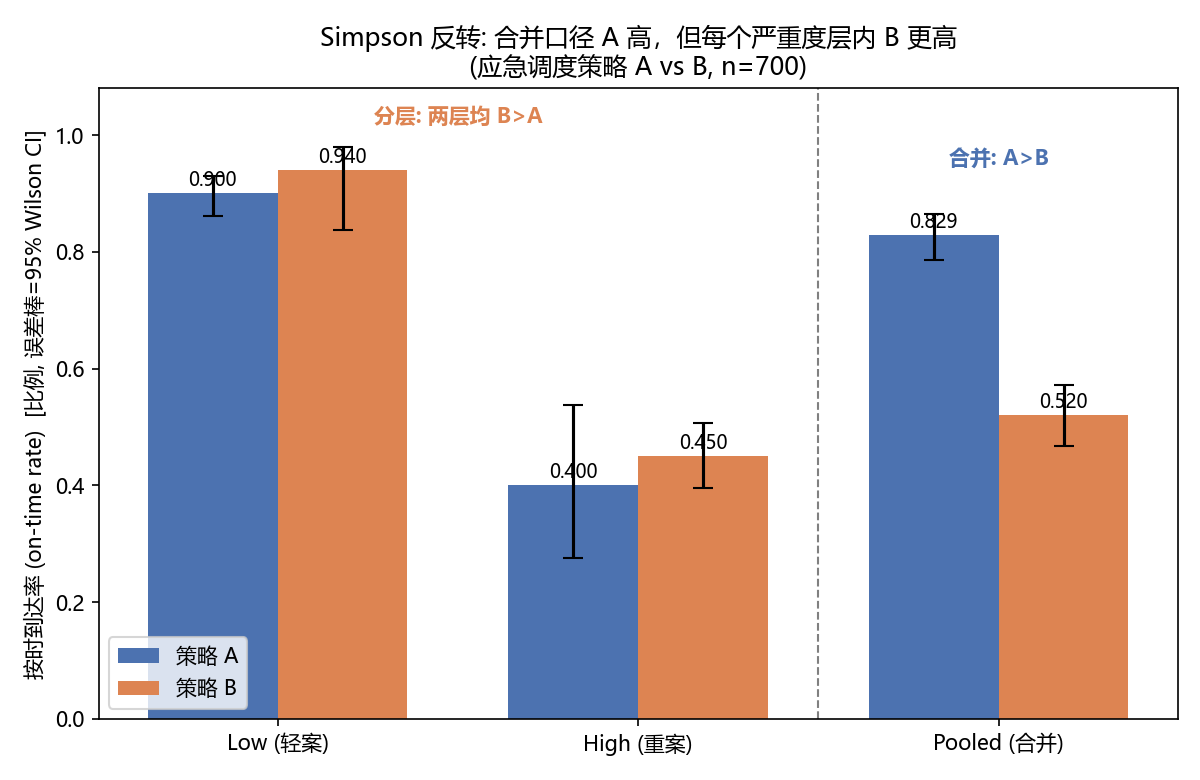
\includegraphics[width=0.85\textwidth]{figures/fig1_simpson_reversal.png}
\caption{合并 vs 分层按时率对比：最右``合并''柱 A 高于 B，而 Low、High 两组层内柱均 B 高于 A，方向反转一目了然（误差棒为 95\% Wilson CI）。}
\end{figure}

\textbf{不确定性如实交代}：两层内差的 95\% CI 均跨 0（Low $[-0.114,+0.034]$、High $[-0.197,+0.097]$）。反转方向稳定（两层点估计均 B 高），但单层``B 高''在统计上不显著——最小格 $n=50$ 使单层 CI 偏宽。反转作为``现象''成立；``B 在某层显著更优''则证据不足。

\begin{figure}[htbp]
\centering
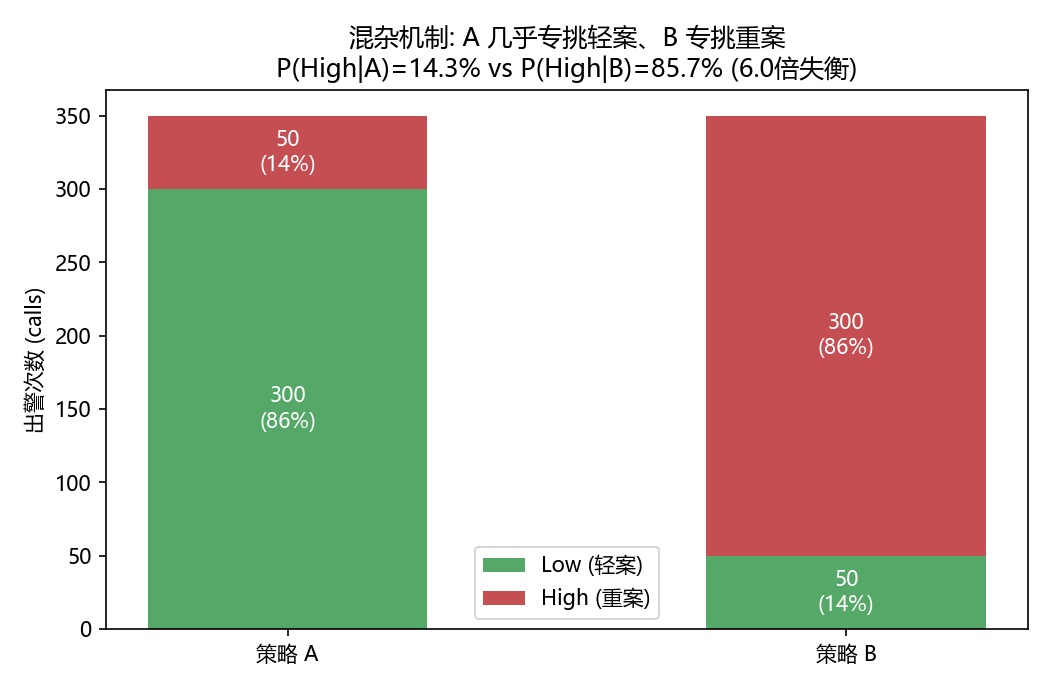
\includegraphics[width=0.85\textwidth]{figures/fig2_confounding_imbalance.png}
\caption{混杂机制：A 接重案仅 14.3\%、B 接重案达 85.7\%（失衡 6.0 倍）。两策略几乎没接到同类难度构成的呼叫，合并率把案件难度差误算成策略效果差。}
\end{figure}

混杂机制：A 接重案仅 14.3\%、B 接重案达 85.7\%，失衡 \textbf{6.0 倍}；\texttt{severity} 边际效应 $P(Y|L)-P(Y|H)=0.9057-0.4429=0.4629$。这是本案最扎实、最可解释的发现。

\subsection{Q3 · 公平比较三法（控制 severity）}
\textbf{(a) 直接标准化率差}（主权重 = 总体权 0.5/0.5）：标准化率 A$=0.6500$、B$=0.6950$，\textbf{B 较 A 优 $+4.5$ pp}，95\% bootstrap CI $[-3.83,+12.67]$ pp（含 0）。

\textbf{(b) Mantel--Haenszel 合并 OR}：\textbf{OR(A/B)$=0.7527$}（$<1$ $\to$ B 优），95\% CI $[0.4378,1.2941]$（含 1）；Breslow--Day $\chi^2=0.2525$（$p=0.6154$）$\to$ 层间 OR 同质。

\textbf{(c) logistic 回归}（A,Low 为参照）：
\begin{center}
\begin{tabular}{lcccc}
\toprule
系数 & 估计 & OR & 95\% CI(OR) & $p$ \\
\midrule
policy=B（控制 severity） & $\beta_1=+0.2799$ & \textbf{1.3230} & $[0.7728,2.2650]$ & \textbf{0.3075} \\
severity=High & $\beta_2=-2.6964$ & 0.0675 & --- & $<10^{-15}$ \\
\bottomrule
\end{tabular}
\end{center}
OR(B/A)$=1.323>1$（B 几率更高），与 MH 互印证（$1/0.7527=1.329\approx1.323$，方向对齐正确）；交互项 $p=0.617$（不显著）$\to$ 无显著效应异质性，与 Breslow--Day 一致。

\begin{figure}[htbp]
\centering
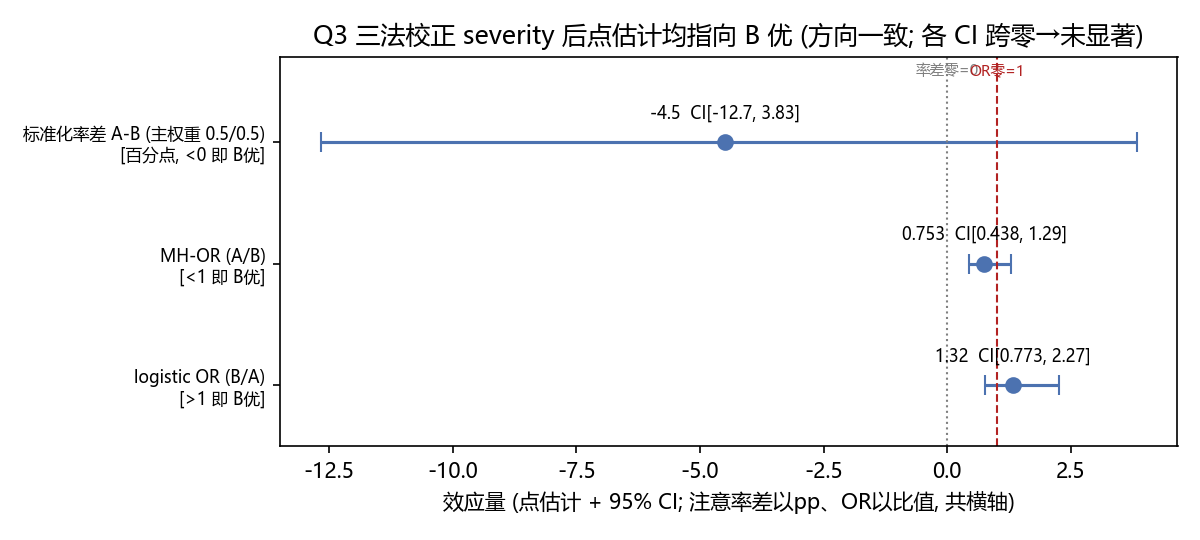
\includegraphics[width=0.8\textwidth]{figures/fig3_three_methods_forest.png}
\caption{三法森林图：标准化率差、MH-OR、logistic OR 点估计方向一致地指向 B 略优，但 95\% 区间均跨过各自零值。}
\end{figure}

\begin{center}
\begin{tabular}{lcc}
\toprule
方法 & 统计量 & 指向 B 优？ \\
\midrule
(a) 标准化率差（主权重） & A$-$B $=-4.5$ pp $<0$ & 是 \\
(b) MH-OR(A/B) & $0.7527<1$ & 是 \\
(c) logistic OR(B/A) & $1.323>1$ & 是 \\
\bottomrule
\end{tabular}
\end{center}
\textbf{三法点估计方向一致地指向 B 略优。但三法的 95\% 区间均跨过各自零值（率差含 0、OR 含 1、logistic $p=0.31$），无一达 $\alpha=0.05$。} 故唯一可防守的结论是：\textbf{校正 severity 后，B 不劣于 A、点估计略优约 4--5 pp，但在 $n=700$、最小格 $n=50$ 下未达统计显著；据此不足以让市政在 A/B 间做出有把握的优选，但足以证明``用合并率推荐 A''是错误方向}。三法是同一批数据的三种换算，并非三份独立证据，不能用``方向一致''反推``统计显著''。

\section{灵敏度分析}
\begin{center}
\begin{tabular}{p{2.6cm}p{2.6cm}p{4.5cm}p{3cm}}
\toprule
维度 & 设置 & 结果 & 稳健性 \\
\midrule
标准化权重 & 总体 / A 人群 / B 人群 & A$-$B $\in[-4.86,-4.14]$ pp，恒为负，漂移约 0.7 pp & 方向稳健，强度不敏感 \\
层间效应同质 & Breslow--Day + 交互项 & $p=0.6154$ / $p=0.6170$，均不显著 & 同质成立，合并 OR 可用 \\
最小格样本 & High-A、Low-B 各 $n=50$ & 单层差 CI 偏宽、跨 0 & 反转方向稳，显著性不足 \\
severity 边际效应 & $P(Y|L)-P(Y|H)$ & 0.4629 & 混杂确强 \\
bootstrap 复现 & seed=42 重跑 & 数值逐位一致 & 可复现 \\
\bottomrule
\end{tabular}
\end{center}
核心结论：\textbf{``校正后 B 略优''的方向对权重和层间同质假设都稳健（漂移仅 0.7 pp、两项同质检验均不显著）；但所有不确定性区间都跨零，强度上的``不显著''也同样稳健}——稳健的是方向，不是显著性。

\section{模型的评价}
\subsection{优点}
(1) 叙事链完整且可证伪：Q1（陷阱）$\to$ Q2（反转判定准则，0/1 可判定）$\to$ Q3（三法校正），每步配``为什么选它''与代价。(2) 三法交叉印证 + 数值互验：MH-OR 倒数 $1/0.7527=1.329$ 与 logistic OR 1.323 互验，编码方向对齐正确。(3) 敏感性扎实：三套权重、双查同质、最小格标注、bootstrap 1 万次，全部可复现。(4) 创新落点可被引用：``难度配平比较法''把``公平=同等难度下比''讲成市政能懂的一句话。

\subsection{局限性（如实写入 Critic 审计裁决）}
本文严守独立审计（Critic）红线，不藏短板：
\begin{enumerate}
\item \textbf{效应未达统计显著（最重要的诚实）}：三法 95\% 区间均跨零（率差含 0、MH-OR 含 1、logistic $p=0.31$），两层内差也都不显著（Low $p=0.290$、High $p=0.505$）。故\textbf{``B 显著优于 A / 推荐市政采用 B / B 胜出''在本数据下不成立}；本文只主张``校正后 B 不劣于、点估计略优、未达显著''。
\item \textbf{不可声称因果}：数据仅 3 字段，时段/路况/警力等未观测混杂无法排除（A1），\texttt{severity} 判定是否独立于 \texttt{policy} 数据内无法验证（A5）。所有结论仅在``给定可观测 severity 下、关联层面''成立，\textbf{不得写``B 导致更高按时率''}。
\item \textbf{样本量与功效}：效应量小（约 4--5 pp / OR$\approx$1.32），最小格 $n=50$，功效不足；``五个角度点估计同号''在效应方向一致而强度微弱时本就常见，不等于显著。
\item \textbf{外推受限}：样本为试点期记录，无时间/区域字段，选择偏差无法验证（A4）。
\item \textbf{口径未核实项}：\texttt{on\_time} 跨策略时限一致性（A3）、\texttt{severity} 判定独立性（A5）数据内均无法证伪，仅能标注待核实。
\end{enumerate}

\subsection{本案自纠留痕}
本案由 ModelCrew 子代理端到端真跑。Critic 不信任散文，\textbf{独立写脚本从原始 CSV 重算全部关键量}逐项核对 \texttt{results.json}：所有数字经得起独立复算，无造假、无除零、无 NaN，反转真实成立。同时揪出早期散文 \texttt{4\_results.md} 中 3 处旧版残留数字（logistic $\beta_{sevH}$ 旧值 $-2.494$ 应为 $-2.6964$、交互项 $p$ 旧值 0.964 应为 0.617、A 的 Wilson CI 旧值 $[0.7847,0.8650]$ 应为 $[0.7856,0.8644]$），已据 \texttt{results.json} 为唯一真值同步修正；三处均不改变任何结论方向。本文所有数字与 \texttt{frozen\_numbers.json} / \texttt{results.json} 同源。

\subsection{改进方向}
采集并纳入时段、路况、出动警力等候选混杂做更充分的回归调整或倾向得分匹配；若条件允许，\textbf{对呼叫做随机化派遣}可从根本上消除混杂、支持因果结论；扩大样本量以提升对约 4--5 pp 小效应的统计功效。

\section{结论}
(1) \textbf{Q1 的合并率是陷阱，不可据此推荐 A}：合并按时率 A$=0.8286$ 远高于 B$=0.5200$，但这是 A 专挑轻案、B 专挑重案（失衡 6.0 倍）造成的混杂假象。(2) \textbf{Q2 混杂确实导致误判，Simpson 反转真实发生}：分层后两层内均 B 高于 A，与合并方向相反；但单层``B 高''未达统计显著。(3) \textbf{Q3 公平比较应控制 severity}：三法点估计一致指向 B 略优（约 4--5 pp / OR$\approx$1.32），方向对权重稳健，\textbf{但效应未达统计显著}。

\textbf{给市政的可落地建议}（仅由结果支持的两条）：

\begin{itemize}
\item \textbf{不要用合并按时率在 A、B 间做优选}——它会因案件难度构成不同而系统性误导，几乎确定推荐错策略。
\item \textbf{公平比较必须在同等案件难度（severity）下进行}（``难度配平比较法''）：用标准化率 / 合并 OR / 回归调整校正后再比。在此口径下现有证据\textbf{不足以判定 B 显著优于 A}，故暂不宜替市政在 A/B 间下定论；若要做出有把握的优选，建议采集更多协变量、扩大样本，或直接对呼叫随机化派遣后重评。
\end{itemize}

\begin{thebibliography}{9}
\bibitem{simpson1951} Simpson, E. H. The Interpretation of Interaction in Contingency Tables. \textit{Journal of the Royal Statistical Society, Series B}, 1951, 13(2): 238--241.
\bibitem{mh1959} Mantel, N., Haenszel, W. Statistical Aspects of the Analysis of Data from Retrospective Studies of Disease. \textit{Journal of the National Cancer Institute}, 1959, 22(4): 719--748.
\bibitem{rothman2008} Rothman, K. J., Greenland, S., Lash, T. L. \textit{Modern Epidemiology}. 3rd ed. Lippincott Williams \& Wilkins, 2008.
\bibitem{agresti2013} Agresti, A. \textit{Categorical Data Analysis}. 3rd ed. Wiley, 2013.
\end{thebibliography}

\appendix
\section{附录}
\textbf{复现信息}：代码 \texttt{solve.py}（\texttt{python solve.py}，绝对路径定位数据）；数据 \texttt{data/dispatch.csv}，MD5$=$\texttt{496fd5aafdbbcc3f11edba376d5f2331}（运行时实时校验）；随机种子 \texttt{seed=42}，bootstrap \texttt{N\_BOOT=10000}（\texttt{numpy.random.default\_rng(42)}，分层 4 格各自有放回重采样）。CI 方法：单比例 Wilson；两比例差 Wald；标准化率差 bootstrap 百分位；MH-OR Robins--Breslow--Greenland 方差；logistic Wald CI。图：\texttt{figures/fig1\_simpson\_reversal.png}、\texttt{fig2\_confounding\_imbalance.png}、\texttt{fig3\_three\_methods\_forest.png}。数字唯一真值源：\texttt{frozen\_numbers.json} / \texttt{results.json}。

\noindent\textbf{产出说明}：本文由 ModelCrew 子代理端到端真跑产出（Router 定题 $\to$ Analyst 审题 $\to$ Scout 数据体检 $\to$ Modeler 选模型 $\to$ Solver 真跑求解 $\to$ Critic 独立复算审计 $\to$ Writer 成稿）。所有数字与 \texttt{frozen\_numbers.json} / \texttt{results.json} 同源，未另造。本 \texttt{.tex} 已用 \textbf{MiKTeX xelatex 编译通过}（\texttt{6\_paper.pdf}，13 页，无未定义引用）；复现：\texttt{xelatex 6\_paper.tex}（跑两遍）。

\end{document}
